\begin{figure}[H] 
  \begin{subfigure}[b]{0.5\linewidth}
    \centering
    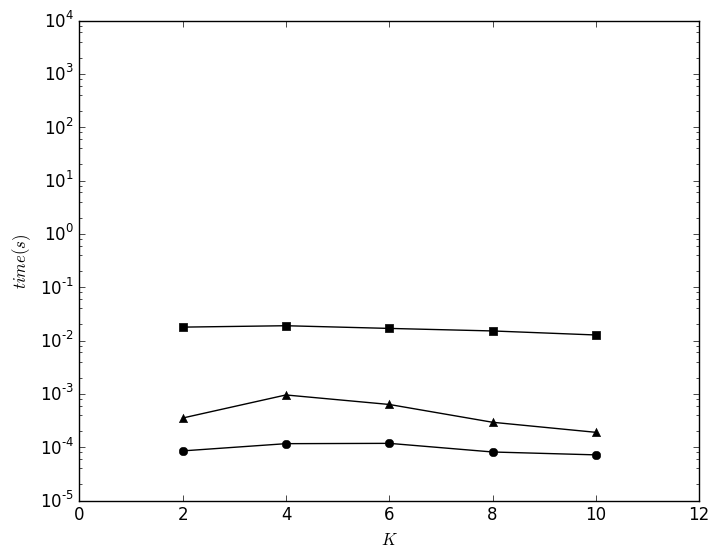
\includegraphics[width=0.9\linewidth]{Pictures/n10} 
    \caption{$N=10$} 
    \label{fig:fixed_n:a} 
    \vspace{4ex}
  \end{subfigure}%% 
  \begin{subfigure}[b]{0.5\linewidth}
    \centering
    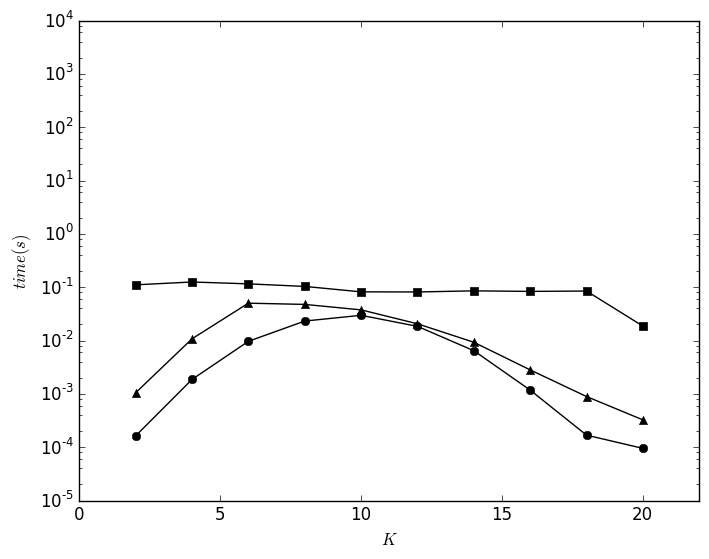
\includegraphics[width=0.9\linewidth]{Pictures/n20} 
    \caption{$N=20$} 
    \label{fig:fixed_n:b} 
    \vspace{4ex}
  \end{subfigure} 
  \begin{subfigure}[b]{0.5\linewidth}
    \centering
    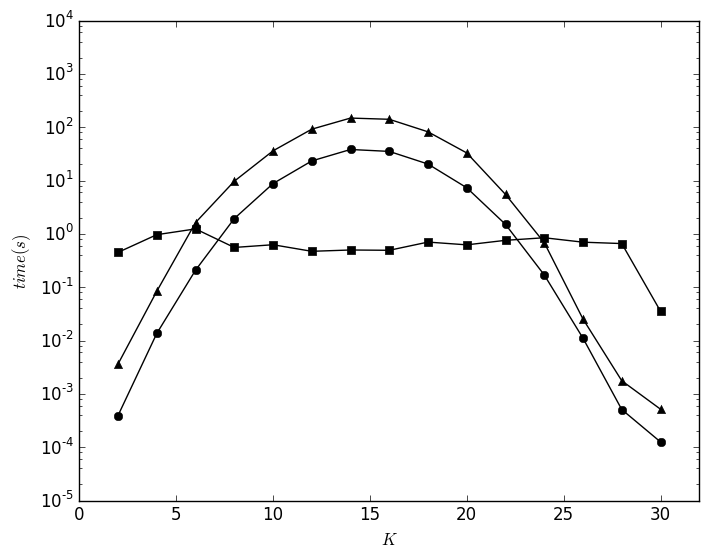
\includegraphics[width=0.9\linewidth]{Pictures/n30} 
    \caption{$N=30$} 
    \label{fig:fixed_n:c} 
  \end{subfigure}%%
  \begin{subfigure}[b]{0.5\linewidth}
    \centering
    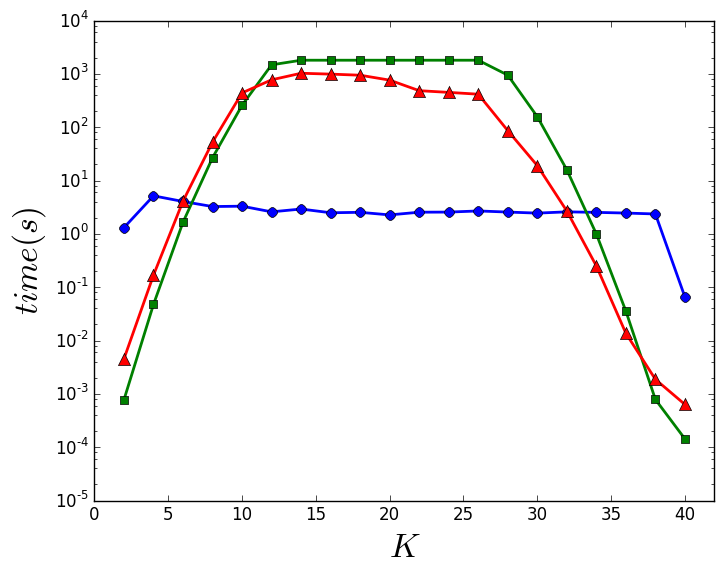
\includegraphics[width=0.9\linewidth]{Pictures/n40} 
    \caption{$N=40$} 
    \label{fig:fixed_n:d} 
  \end{subfigure} 
  \vspace{2ex}
  \smark\ -- Integer Linear Programming, \tmark\ -- Delaunay Assisted BB, \cmark\ -- Branch-and-bound
  \caption{Result times for different values of $N$ with varying $K$}
  \label{fig:fixed_n} 
\end{figure}

